\documentclass[tikz]{standalone}
\usepackage{amsmath,amssymb}
\usetikzlibrary{arrows.meta,positioning,fit,calc,decorations.pathreplacing,shapes.geometric}

\begin{document}
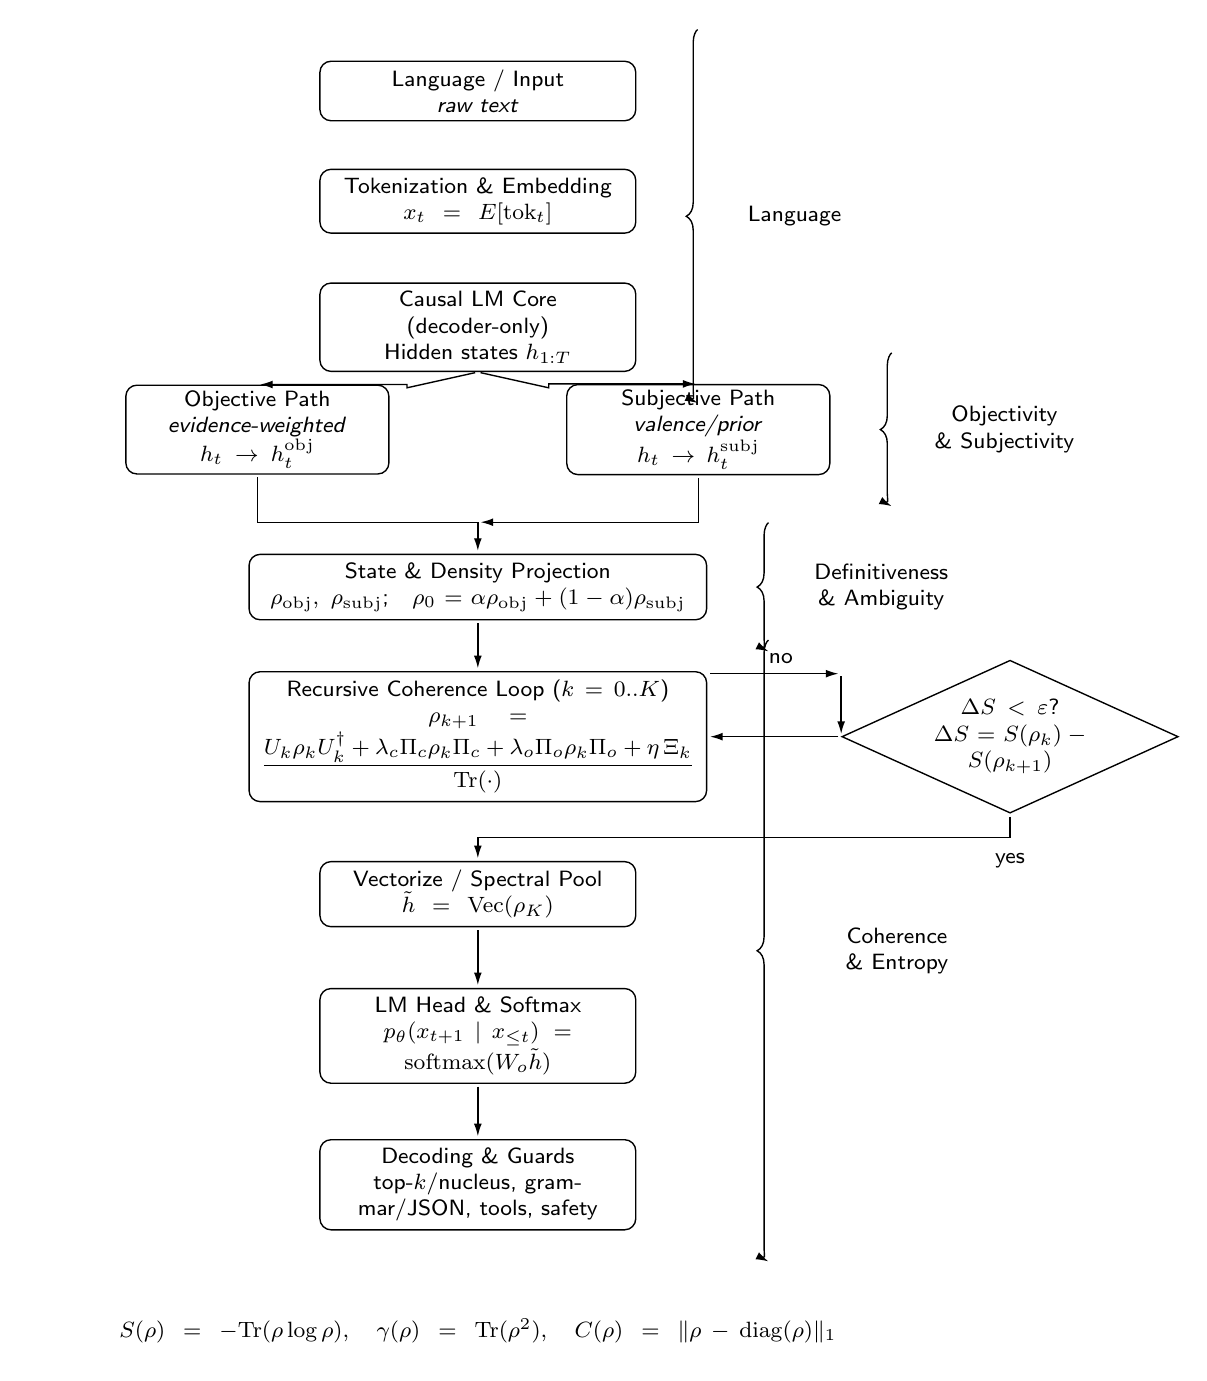
\begin{tikzpicture}[
  font=\sffamily\footnotesize,
  node distance=6mm and 8mm,
  >=LaTeX,
  every path/.style={line width=0.5pt, -{Latex[length=1.6mm,width=1mm]}, shorten >=1pt, shorten <=1pt},
  block/.style={draw, rounded corners, align=center, inner sep=3pt, minimum height=7mm, text width=38mm},
  nwide/.style={draw, rounded corners, align=center, inner sep=3pt, minimum height=7mm, text width=56mm},
  tinyb/.style={draw, rounded corners, align=center, inner sep=2pt, minimum height=7mm, text width=32mm},
  decision/.style={draw, shape=diamond, aspect=2.2, inner sep=0pt, align=center, minimum height=7mm, text width=22mm},
  stagelabel/.style={align=center}
]

% ----- Fixed coordinates for tidy layout
\coordinate (X1) at (0,0);
\coordinate (X2) at (0,-1.4);
\coordinate (X3) at (0,-3.0);
\coordinate (X4) at (0,-6.3);
\coordinate (X5) at (0,-8.2);
\coordinate (X6) at (0,-10.2);
\coordinate (X7) at (0,-12.0);

\coordinate (Lcol) at (-2.8,-4.3);
\coordinate (Rcol) at ( 2.8,-4.3);

% ----- Main engine
\node[block] at (X1) (input) {Language / Input\\\emph{raw text}};
\node[block] at (X2) (tok) {Tokenization \& Embedding\\$x_t=E[\mathrm{tok}_t]$};
\node[block] at (X3) (enc) {Causal LM Core (decoder-only)\\Hidden states $h_{1:T}$};

% ----- Objective / Subjective parallel heads
\node[tinyb] at (Lcol) (obj) {Objective Path\\\emph{evidence-weighted}\\$h_t\!\to\!h^{\mathrm{obj}}_t$};
\node[tinyb] at (Rcol) (subj) {Subjective Path\\\emph{valence/prior}\\$h_t\!\to\!h^{\mathrm{subj}}_t$};

% Fan-out from core to two heads (orthogonal)
\path (enc.south) ++(-0.9,-0.2) coordinate (tapL);
\path (enc.south) ++( 0.9,-0.2) coordinate (tapR);
\draw (enc.south) -- (tapL) |- (obj.north);
\draw (enc.south) -- (tapR) |- (subj.north);

% ----- Density projection / fusion
\node[nwide] at (X4) (rho) {State \& Density Projection\\
$\rho_{\mathrm{obj}},\ \rho_{\mathrm{subj}}$;\quad
$\rho_0=\alpha\rho_{\mathrm{obj}}+(1-\alpha)\rho_{\mathrm{subj}}$};

\path ($(obj.south)!0.5!(subj.south)$) ++(0,-0.6) coordinate (midJ);
\draw (obj.south) |- (midJ) -- (rho.north);
\draw (subj.south) |- (midJ);

% ----- Recursive core
\node[nwide] at (X5) (rci) {Recursive Coherence Loop ($k=0..K$)\\
$\displaystyle \rho_{k+1}=\frac{U_k\rho_k U_k^\dagger+\lambda_c \Pi_c\rho_k\Pi_c+\lambda_o \Pi_o\rho_k\Pi_o+\eta\,\Xi_k}{\mathrm{Tr}(\cdot)}$};
\draw (rho) -- (rci);

% ----- Halting decision
\node[decision, right=17mm of rci] (halt) {$\Delta S < \varepsilon$?\\ $\Delta S=S(\rho_k)-S(\rho_{k+1})$};

% Bottom horizontal line FLIPPED: arrowhead points from diamond -> RCI (same length)
\draw (halt.west) -- (rci.east);

% ----- NO loop (same length as bottom line; starts at RCI; ends aligned with halt.west)
\def\NoGap{8mm} % increase/decrease this to adjust the vertical gap

\coordinate (topStart) at ($(rci.east)+(0,\NoGap)$);
\coordinate (topEnd)   at ($(halt.west)+(0,\NoGap)$);

% Top horizontal arrow (RCI -> diamond) + label above it
\draw (topStart) -- (topEnd) node[above,pos=0.55]{no};

% Vertical (perpendicular) downward arrow connecting top and bottom at the SAME x (halt.west)
\draw (topEnd) -- (halt.west);

% --- YES path: straight down to projection
\node[stagelabel] at ($(halt.south)+(0,-6mm)$) {yes};
\node[block]  at (X6) (proj) {Vectorize / Spectral Pool\\$\tilde{h}=\mathrm{Vec}(\rho_K)$};
\draw (halt.south) |- ++(0,-3mm) -| (proj.north);

% ----- LM head and decoding
\node[block]  at (X7) (lm) {LM Head \& Softmax\\$p_\theta(x_{t+1}\!\mid\!x_{\le t})=\mathrm{softmax}(W_o \tilde{h})$};
\draw (proj) -- (lm);

\node[block, below=7mm of lm] (decode) {Decoding \& Guards\\top-$k$/nucleus, grammar/JSON, tools, safety};
\draw (lm) -- (decode);

% ----- Stage braces on the RIGHT (avoid crossings)
\node[fit=(input)(tok)(enc), inner sep=2mm] (G1) {};
\node[fit=(obj)(subj), inner sep=2mm] (G2) {};
\node[fit=(rho), inner sep=2mm] (G3) {};
\node[fit=(rci)(proj)(lm)(decode), inner sep=2mm] (G4) {};

\draw[decorate,decoration={brace,mirror,amplitude=5pt}]
  ($(G1.north east)+(6mm,2mm)$) -- ($(G1.south east)+(6mm,-2mm)$)
  node[midway,xshift=12mm,align=center] {Language};

\draw[decorate,decoration={brace,mirror,amplitude=5pt}]
  ($(G2.north east)+(6mm,2mm)$) -- ($(G2.south east)+(6mm,-2mm)$)
  node[midway,xshift=14mm,align=center] {Objectivity\\\& Subjectivity};

\draw[decorate,decoration={brace,mirror,amplitude=5pt}]
  ($(G3.north east)+(6mm,2mm)$) -- ($(G3.south east)+(6mm,-2mm)$)
  node[midway,xshift=14mm,align=center] {Definitiveness\\\& Ambiguity};

\draw[decorate,decoration={brace,mirror,amplitude=5pt}]
  ($(G4.north east)+(6mm,2mm)$) -- ($(G4.south east)+(6mm,-2mm)$)
  node[midway,xshift=16mm,align=center] {Coherence\\\& Entropy};

% ----- Compact footer (no wrapping)
\node[align=center, text width=112mm, below=10mm of decode] (defs)
  {$S(\rho)=-\mathrm{Tr}(\rho\log\rho),\quad \gamma(\rho)=\mathrm{Tr}(\rho^2),\quad C(\rho)=\|\rho-\mathrm{diag}(\rho)\|_1$};

\end{tikzpicture}
\end{document}




